\documentclass[11pt,a4paper]{article}
\usepackage{theme/lmuthesis}

\usepackage[T1]{fontenc}
\usepackage[english]{babel}
\usepackage{unicode-math}
\usepackage{amsmath, amsfonts}
\usepackage{wasysym}
\usepackage{amsthm, thmtools}
\declaretheorem[numberwithin=section]{lemma, proposition, theorem}
\declaretheorem[numberwithin=section, style=plain]{example}
\declaretheorem[style=definition, numberwithin=section]{definition}
\declaretheorem[style=remark, numberwithin=section]{remark}

\usepackage{epstopdf}
\usepackage{tikz}
\usepackage{pgfplots}

\usepackage{physics}

% this for draft water mark
\setboolean{release}{true}
\IfFileExists{condition}{\input{condition}}{}
\ifthenelse{\boolean{release}}{
}{
    \usepackage{draftwatermark}
    \SetWatermarkText{DRAFT}
    \SetWatermarkScale{1}
}

% meta informations
\department{Institut für TODO}
\lfe{Lehr- und Forschungseinheit TODO}
\professor{Prof.\ Dr.\ PROFESSORS NAME}
\type{Bachelor's Thesis}
\title{THESIS TITLE}
\author{Valentin Herrmann}
\email{EMAIL}
\bearbeitungszeitraum{START bis END}
\supervisor{SUPERVISOR}
\taskdescription{
    \begin{description}
        \item[THESIS TITLE]
        \item[Problem Statement] TO BE ADDED
        \item[Scope of the Thesis] TO BE ADDED
        \item[Tasks] TO BE ADDED
        \item[Requirements] TO BE ADDED
        \item[Keywords] TO BE ADDED
    \end{description}
}
\acknoledgement{
    I would like to appreciate ...
}
\abstract{
    This thesis proposes ...
}

\newcommand{\dtlifsnn}{r. d.t. LIF-SNN }
\newcommand{\Dtlifsnn}{R. d.t. LIF-SNN }
\newcommand{\proofofref}[1]{Proof of~\autoref{#1}.}

\begin{document}

\makecover
\maketaskdescription
\makededication
\makeabstract
\maketoc
% optional:
% \listoffigures
% \listoftables
\cleardoublepage

\section{Introduction}
\label{ch:intro}

While the hype on AI is still ongoing there are still people wondering if current AI models are fundamentally able of reasoning. Many other possible models could be better fitted to the task of reasoning. Among others Spiking neural networks present a model closer to the workings of the brain. In fact, they have been called the 3rd generation of AI models, after the 2nd generation that currently drives most successful models.

While the idea behind SNNs is quite old, they have not been as much researched, since it is much more inefficient and harder to train them. Therefore there still remain a lot of open questions about them.
In this paper we shall extend on the work done in~\cite{nguyen2025timespikeunderstandingrepresentational}. We will add a decaying factor to the input of the neurons and allow recursive connections between neurons in a layer.

We will roughly follow the structure of~\cite{nguyen2025timespikeunderstandingrepresentational}. In the second chapter we will formally introduce discrete time leaky-integrate-and-fire SNN, d.t. LIF-SNNs. In section 3 we will give theorems about approximation of continuous functions on compact domains by d.t. LIF-SNNs.
The main part will be the following section in which we will see that the number of distinct values a d.t. LIF-SNN can take on only depends on the first hidden layer and grows in particular only quadratically in time. We will further support our findings with experimental data in the last section.
% approximation of differentiable ones?
 \cleardoublepage
\section{Definitions}
\label{ch:defs}

% TODO: graphic for whole layer
Our type of SNN should be thought of as a composition of an initial input layer, a number of hidden spiking layers with internal state and an affine-linear layer mapping spikes activations over time, so called spike trains, to the value of the output layer.
Like motivated we are adding additional structure to the definitions~\cite{nguyen2025timespikeunderstandingrepresentational}.
We shall first define the input \(i^{[l]}(t)\), the membrane potential before spike \(p^{[l]}(t)\), the membrane potential after spike \(u^{[l]}(t)\) and the spike activations \(s^{[l]}(t)\) of the hidden layers:

% TODO: graphic for single neuron/single layer
%TODO: herleitung: ~/Downloads/1901.09948v2.pdf
\begin{definition}
  The \textbf{input vector} \(i^{[l]}(t)∈\{0,1\}^{n_l}\), the \textbf{spike vector} \(s^{[l]}(t)∈\{0,1\}^{n_l}\) and the \textbf{membrane potential vector} \(u^{[l]}(t)\) of a hidden layer \(λ=(W^{[l]},b^{[l]},u^{[l]}(0),i^{[l]}(0),α^{[l]},β^{[l]},ϑ^{[l]})\), \(l∈[L]\), are recursively defined as
  \begin{align}
    i^{[l]}(t) & ≔ α^{[l]}i^{[l]}(t-1)+W^{[l]}s^{{(l)}-1}(t)+V^{[l]}s^{[l]}(t-1) \\
    p^{[l]}(t) & ≔ β^{[l]}u^{[l]}(t-1)+i^{[l]}(t)+b^{[l]} \\
    s^{[l]}(t) & ≔ H(p^{[l]}(t)-ϑ1_{n_l}) \\
    u^{[l]}(t) & ≔ p^{[l]}(t)-ϑs^{[l]}(t)
  \end{align}
  with \(s^{[l]}(0)=0\) and given
  \begin{enumerate}
    \item[•] \textbf{initial membrane potential}: \(u^{[l]}(0)∈ℝ^{n_l}\),
    \item[•] \textbf{initial input}: \(i^{[l]}(0)∈ℝ^{n_l}\),
    \item[•] \textbf{weight matrices}: \(W^{[l]}∈ℝ^{n_l×n_{l-1}}\), \(V^{[l]}∈ℝ^{n_l×n_l}\),
    \item[•] \textbf{bias vectors}: \(b^{[l]}∈ℝ^{n_l}\),
    \item[•] \textbf{leaky terms}: \(α^{[l]},β^{[l]}∈[0,1]\),
    \item[•] \textbf{threshold}: \(ϑ^{[l]}∈(0,∞)\),
  \end{enumerate}
  where \(H≔𝟙_{[0,∞)}\) is a step function and \(T∈ℕ\) is the number of simulated time steps.
\end{definition}

We further define recurrent d.t. LIF-SNN and the function the network realizes:
\begin{definition}
  A \textbf{recurrent discrete-time LIF-SNN} of \textbf{depth} \(L\) with \textbf{layer-widths} \((n_0,…,n_{L+1})\) and \(T∈ℕ\) time-steps is given by
  \[ Φ≔((W^{[l]},b^{[l]},V^{[l]},u^{[l]}(0),i^{[l]}(0),α^{[l]},β^{[l]},ϑ^{[l]})_{l∈[L]},T,(E,D)) \]
  where the \textbf{input encoder} \(E:ℝ^{n_0}→ℝ^{n_0×T}\) maps a vector \(x∈ℝ^{n_0}\) to a corresponding first layer spike activation \(s^{[0]}=E(x)\) and the \textbf{output decoder} \(D:\{0,1\}^{n_L×T}→ℝ^{n_{L+1}}\) maps the spike activations of the last hidden layer to real values.
\end{definition}

% TODO: remark about layers being kinda useless
% TODO: remark comparison with previous model
% TODO: layers mit kursiv?

\begin{definition}
  A recurrent discrete-time LIF-SNN \(ϕ\) \textbf{realizes} the function \(R(Φ):ℝ^{n_0}→ℝ^{n_{L+1}}\):
  \[ R(Φ)(x)=D((s^{[L]}(t))_{t∈[T]})\quad \text{with }s^{[0]}≔E(x)\]
\end{definition}

\begin{definition}
  A recurrent discrete-time LIF-SNN employs \textbf{direct encoding} if we have
  \[ ∀_{t∈[T]}E(x)(t)=x \]
  for the input encoder and has \textbf{membrane potential outputs} if the output decoder can be written as
  \[ D((s(t))_{t∈[T]})=\sum_{t=1}^Ta_t(W^{[L+1]}s(t)+b^{[L+1]}) \]
  for some \((a_t)_{t∈[T]}∈ℝ^T\), \(b^{[L+1]}∈ℝ^{n_{L+1}}\) and \(W^{[L+1]}∈ℝ^{n_{L+1}×n_L}\).
\end{definition}
We will only consider recurrent discrete-time LIF-SNN with direct encoding and membrane potential outputs. In fact, we will use “recurrent discrete-time LIF-SNN” to mean “\rdtlifsnn with direct encoding and membrane potential”.

For clearer construction of our networks we will additionally define neurons:

% TODO: just notation?
\begin{definition}
  The \(i\)-th neuron of a hidden layer \(λ=(W^{[l]},b^{[l]},V^{[l]},u^{[l]}(0),i^{[l]}(0),α^{[l]},β^{[l]},ϑ^{[l]})\) of a \rdtlifsnn is a tuple \((w,b,v,u_0,i_0)\) with \(w∈ℝ^{n_{l-1}}\), \(v∈ℝ^{n_l}\) and \(b,u_0,i_0∈ℝ\), such that \(b\), \(u_0\), \(i_0\) are the \(i\)-th component of \(b^{[l]}\), \(u^{[l]}(0)\), \(i^{[l]}(0)\) respectively and \(w\), \(v\) are the \(i\)-th row vector of \(W^{[l]}\), \(V^{[l]}\) respectively.
\end{definition}

The following lemmas will be very helpful for the proofs in the following sections:
\begin{lemma}\label{lem:non-recursive-defs}
  We define the following non-recursive formulas with explicit reference to the previous spikes. Let \(1≤t≤T\) and \((s_p^{[l]})_{l∈\{0…L'\}}\) such that \(s_p^{[l]}:\{0,1\}^{n_l×t'_l}\) for \(l∈\{0…L'\}\). \(L'\) and \(∀_lt'_l\) have to be chosen such that the following terms are well-defined, e.g. \(L'=L\) and \(∀_lt'_l=T\)
  \begin{align}
   i^{[l]}(t;(s_p^{[l]})_l)&≔(α^{[l]})^ti^{[l]}(0)+\sum_{k=1}^t(α^{[l]})^{t-k}\left(W^{[l]}s_p^{[l-1]}(k)+V^{[l]}s_p^{[l]}(k-1)\right), \\
   p^{[l]}(t;(s_p^{[l]})_l) &≔ (β^{[l]})^tu^{[l]}(0)+\sum_{k=1}^t(β^{[l]})^{t-k}\left(i^{[l]}(k;(s_p^{[l]})_l)+b^{[l]}\right)-ϑ\sum_{k=1}^{t-1}(β^{[l]})^{t-k}s_p^{[l]}(k),\\
   s^{[l]}(t;(s_p^{[l]})_l) & ≔ H(p^{[l]}(t;(s_p^{[l]})_l)-ϑ1_{n_l}) \\
   u^{[l]}(t;(s_p^{[l]})_l) &≔ (β^{[l]})^tu^{[l]}(0)+\sum_{k=1}^t(β^{[l]})^{t-k}\left(i^{[l]}(k;s_p)+b^{[l]}-ϑs_p^{[l]}(k)\right),
  \end{align}
  We use the convention \(∀_{α,β∈[0,1]}α^0,β^0=1\). These formulas are equivalent to the previous recursive definitions, given \(s_p^{[l]}=s^{[l]}\) for \(l∈\{0…L'\}\).
\end{lemma}

\begin{proof}
  Let the time \(1≤t≤T\) be non-zero. By induction we immediately get
  \[ i^{[l]}(t)=(α^{[l]})^ti^{[l]}(0)+\sum_{i=1}^t(α^{[l]})^{t-i}\left(W^{[l]}s^{[l-1]}(i)+V^{[l]}s^{[l]}(i-1)\right) \]
  By definition of \(u^{[l]}\) and \(p^{[l]}\) we further obtain
  \[ u^{[l]}(t) = β^{[l]}u^{[l]}(t-1)+i^{[l]}(t)+b^{[l]}-ϑs^{[l]}(t) \]
  from which
  \[ u^{[l]}(t) = (β^{[l]})^tu^{[l]}(0)+\sum_{i=1}^t(β^{[l]})^{t-i}\left(i^{[l]}(i)+b^{[l]}-ϑs^{[l]}(i)\right) \]
  follows by induction.
  By substituting \(u^{[l]}\) in \(p^{[l]}\) we further obtain:
  \[ p^{[l]}(t) = (β^{[l]})^tu^{[l]}(0)+\sum_{i=1}^t(β^{[l]})^{t-i}\left(i^{[l]}(i)+b^{[l]}\right)-ϑ\sum_{i=1}^{t-1}(β^{[l]})^{t-i}s^{[l]}(i) \]
\end{proof}

\begin{lemma}\label{lem:sum-spikes-over-time}
  Let \(t_0,t_{ω}∈[T]\) and \(j∈[n_l]\) for an \(l∈[L]\) such that \(t_0≤t_{ω}\). If \(∀_{t∈\{t_0…t_{ω}\}}i^{[l]}_j(t)+b^{[l]}_j≤ϑ\) and \(u^{[l]}_j(t_0-1)<ϑ\), then \(∀_{t∈\{t_0…t_{ω}\}}u^{[l]}_j(t)<ϑ\).

  If further \(β=1\) and \(u^{[l]}_j(t_0-1)+\sum_{t=t_0}^{t_{ω}}(i^{[l]}_j(t)+b^{[l]}_j)≥0\)
  \[ \left( u^{[l]}_j(t_0-1)+\sum_{t=t_0}^{t_{ω}}(i^{[l]}_j(t)+b^{[l]}_j) \right) - ϑ\sum_{t=t_0}^{t_{ω}}s^{[l]}_j(t) <ϑ \]
  If either \(∀_{t∈\{t_0…t_{ω}\}}s^{[l]}_j(t)=0\) or \(∀_{t∈\{t'…t_{ω}\}}i^{[l]}_j(t)+b^{[l]}_j≥0\), where \(t'\) is the latest time \(≤t_{ω}\) such that \(s^{[l]}_j(t')=0\), then we even get
  \[ 0≤\left( u^{[l]}_j(t_0-1)+\sum_{t=t_0}^{t_{ω}}(i^{[l]}_j(t)+b^{[l]}_j) \right) - ϑ\sum_{t=t_0}^{t_{ω}}s^{[l]}_j(t) \]
\end{lemma}

\begin{remark}
  If \(ϑ=1\), we get in particular
  \[ \left\lfloor u^{[l]}_j(t_0-1)+\sum_{t=t_0}^{t_{ω}}(i^{[l]}_j(t)+b^{[l]}_j) \right\rfloor = \sum_{t=t_0}^{t_{ω}}s^{[l]}_j(t) \]
\end{remark}

\begin{proof}
  We proof the first part by induction: Let \(t∈\{t_0…t_{ω}\}\). By definition of \(p^{[l]}\), by the given assumptions and by induction hypothesis we have
  \[ p^{[l]}_j(t)=β^{[l]}u^{[l]}_j(t-1)+i^{[l]}_j(t)+b^{[l]}_j ≤ u^{[l]}_j(t-1)+i^{[l]}_j(t)+b^{[l]}_j<2ϑ  \]
  By definition of \(u^{[l]}\) and \(s^{[l]}\), we further get \(u^{[l]}_j(t)<ϑ\).

  Let us further assume \(β=1\) and \(u^{[l]}_j(t_0-1)+\sum_{t=t_0}^{t_{ω}}(i^{[l]}_j(t)+b^{[l]}_j)≥0\).
  We now get
  \[ u^{[l]}(t_{ω}) = u^{[l]}(t_0-1)+\sum_{k=t_0}^{t_{ω}}\left(i^{[l]}(k)+b^{[l]}-ϑs^{[l]}(k)\right),  \]
  due to~\autoref{lem:non-recursive-defs}. From which we immediately obtain
  \[ \left( u^{[l]}_j(t_0-1)+\sum_{t=t_0}^{t_{ω}}(i^{[l]}_j(t)+b^{[l]}_j) \right) - ϑ\sum_{t=t_0}^{t_{ω}}s^{[l]}_j(t) <ϑ \]
  by the first part of the proof. Let us further proof the left part of the inequality: Let \(t'\) be the latest time that \(s^{[l]}_j(t')=1\) has held for \(t'∈\{t_0…t_{ω}\}\). We may assume that \(t'\) exists since we are otherwise immediately finished. We then get \(ϑ≤p^{[l]}_j(t')\) and therefore
  \[ 0≤u^{[l]}_j(t')=u^{[l]}_j(t_0-1)+\sum_{k=t_0}^{t'}\left(i^{[l]}_j(k)+b^{[l]}_j-ϑs^{[l]}_j(k)\right) \]
  by~\autoref{lem:non-recursive-defs}. By assumption and choice of \(t'\) we can conclude
  \[ ≤u^{[l]}_j(t_0-1)+\sum_{k=t_0}^{t_{ω}}\left(i^{[l]}_j(k)+b^{[l]}_j-ϑs^{[l]}_j(k)\right) \]
\end{proof}

Let us now take a look at some simple examples:

%TODO: examples überarbeiten
\begin{example}
  Let \(T,L∈ℕ\). Then there exists a d.t. LIF-SNN with \(∀_{t∈[T]}s^{[L]}(t)=s^{[0]}(t)\) for any \(s^{[0]}∈\{0,1\}^{n_0×T}\).

  We can proof this by using constant width \(n_l=n\), weights \(W^{[l]}=I_n\), biases \(b^{[l]}=0\), initial membrane potential \(u^{[l]}(0)=0\), leaky term \(β^{[l]}=0\) and threshold \(ϑ^{[l]}=1\) for all \(l∈[L]\).

  We then get by definition:
  \begin{alignat*}{3}
    s^{[l]}(t) & = H(s^{[l-1]}(t)-1_{n_l})  &= \ s^{[l-1]}(t) \\
    u^{[l]}(t) & = \phantom{H(}s^{[l-1]}(t)-s^{[l]}(t)&= 0
  \end{alignat*}
\end{example}

\begin{example}\label{ex:2}
  Let \(T,L∈ℕ\). Then there exists a d.t. LIF-SNN with \(∀_{t∈T}s^{[L]}(t)=\max_{t'∈[t-1]}(s^{[0]}(t'))\) for any \(s^{[0]}∈\{0,1\}^{n_0×T}\): In this network an output neuron switches on when the corresponding input neurons fires and does not switch off later.

  We can proof this by using constant width \(n_l=n\), weights \(W^{[l]}=T·I_n\), biases \(b^{[l]}=0\), initial membrane potential \(u^{[l]}(0)=0\), leaky term \(β^{[l]}=1\) and threshold \(ϑ^{[l]}=1\) for all \(l∈[L]\).

  We then get by definition:
  \begin{alignat*}{2}
    s^{[l]}(t) & = H(&u^{[l]}(t-1)+T·s^{[l-1]}(t)-1_{n_l}) \\
    u^{[l]}(t) & = &u^{[l]}(t-1)+T·s^{[l-1]}(t)-s^{[l]}(t)
  \end{alignat*}
  By adding over all timesteps we obtain
  \begin{alignat*}{1}
    s^{[l]}(t) & = H(T\sum_{i=1}^ts^{[l-1]}(i)-(\sum_{t=i}^{t-1}s^{[l]}(i))+1_{n_l}) ) \\
    u^{[l]}(t) & = \sum_{i=1}^t(T·s^{[l-1]}(i)-s^{[l]}(i))
  \end{alignat*}
  Since \(\sum_{i=1}^{t-1}s^{[l]}(i)+1_{n_l}≤T\), once there is any \(t_0∈[T]\) with \(s^{[l-1]}_i(t_0)=1\) for an \(i\), we get \(∀_{t≥t_0}s^{[l]}_i(t)=1\).
  By induction over the layers we clearly get the required property.
\end{example}
 \cleardoublepage
\section{Structure of computations in \rdtlifsnn s}
\label{ch:struct}

This section concern itself with the approximation of continuous functions by d.t. LIF-SNN.

In~\cite{nguyen2025timespikeunderstandingrepresentational} the following theorem was proved:
\begin{theorem}\label{thm:approx-snn-constant}
  Let \(f\) be a continuous function on a compact set \(Ω⊂ℝ^{n_0}\). For all \(ε>0\), there exists a d.t. LIF-SNN \(Φ\) with direct encoding, membrane potential output, \(L=2\) and \(T=1\) such that
  \[ \norm{R(Φ)-f}_{∞}≤ε\]
  Moreover, if \(f\) is \(Γ\)-Lipschitz, then \(Φ\) can be chosen with width parameter \(n=(n_1,n_2)\) given by
  \begin{align*}
   n_1 &=\left(\max\left\{\left\lceil \frac{\operatorname{diam}_∞(Ω)}{ε}Γ \right\rceil,1\right\}+1\right)n_0  \\
   n_2 &=\max\left\{\left\lceil \frac{\operatorname{diam}_∞(Ω)}{ε}Γ \right\rceil^{n_0},1\right\}
  \end{align*}
  where \(\operatorname{diam}_∞(Ω)=\sup_{x,y∈Ω}\norm{x-y}_∞\).
\end{theorem}

\begin{proof}
  See~\cite{nguyen2025timespikeunderstandingrepresentational}.
\end{proof}

\begin{figure}[h!]
  \begin{subfigure}[t]{0.45\textwidth}
    \centering
    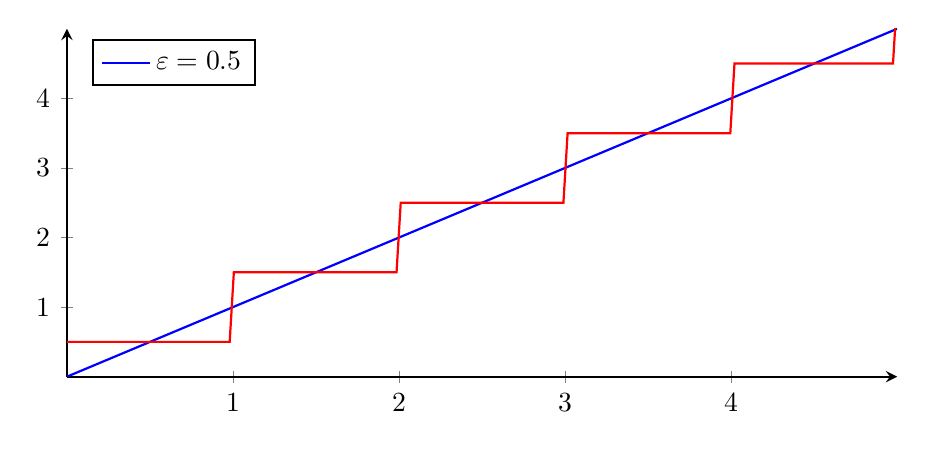
\begin{tikzpicture}
      \begin{axis}[
        axis lines=middle,
        xmin=0, xmax=5,
        ymin=0, ymax=5,
        xtick={0, 1, 2, 3, 4},
        ytick={0, 1, 2, 3, 4},
        domain=0:5,
        samples=200,
        thick,
        legend pos=north west,
        width=\textwidth,
        height=6cm
        ]
        \addplot[blue]{x};
        \addplot[red]{floor(x)+0.5};
        \addlegendentry{$ε=0.5$}
      \end{axis}
    \end{tikzpicture}
    \caption{A \dtlifsnn approximating the identity}
    \label{id:sin-approx-by-dtlifsnn}
  \end{subfigure}
  \hfill
  \begin{subfigure}[t]{0.55\textwidth}
    \centering
    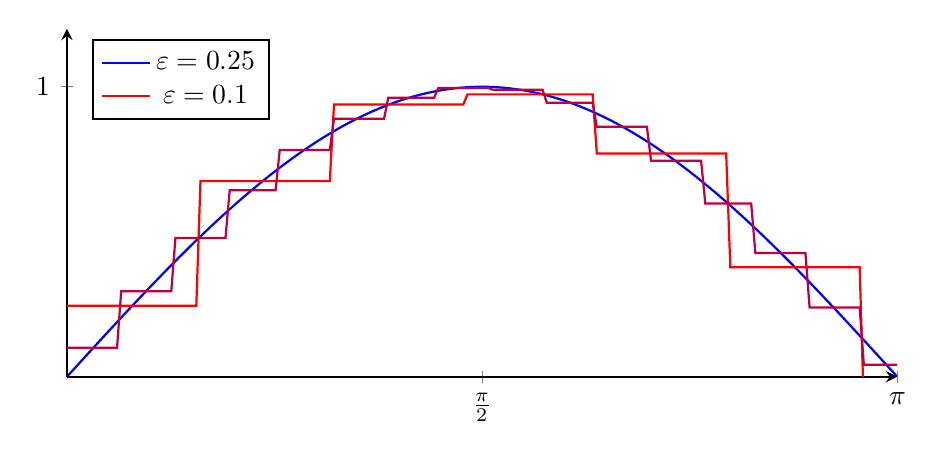
\begin{tikzpicture}
      \begin{axis}[
        axis lines=middle,
        xmin=0, xmax=pi,
        ymin=0, ymax=1.2,
        xtick={0, pi/2, pi},
        xticklabels={$0$, $\frac{\pi}{2}$, $\pi$},
        ytick={0, 1},
        domain=0:pi,
        samples=200,
        thick,
        legend pos=north west,
        width=\textwidth,
        height=6cm
        ]
        \addplot[blue]{sin(deg(x))};
        \addplot[red]{(-cos(deg(floor(x*2+1)/2))+cos(deg(floor(x*2)/2)))*2};
        \addlegendentry{$ε=0.25$} % ε≈0.5*(1/2) (since sin(x)≈x for x≪1)
        \addplot[purple]{(-cos(deg(floor(x*5+1)/5))+cos(deg(floor(x*5)/5)))*5};
        \addlegendentry{$ε=0.1$} % ε≈0.5*(1/5) (since sin(x)≈x for x≪1)
      \end{axis}
    \end{tikzpicture}
    \caption{A \dtlifsnn approximating a sinus wave}
    \label{fig:sin-approx-by-dtlifsnn}
  \end{subfigure}
\end{figure}

The proof of~\autoref{thm:approx-snn-constant} works by first showing that a continuous function can be arbitrarily approximated by step functions, in particular by step functions constant on hypercubes in \(Ω\).
Then the \dtlifsnn is constructed by using the first layer to cut the input space by hyperplanes along the cubes and using the second layer to represent the hypercubes.

While quite simple, this construction does not use the unique feature of (r.) \dtlifsnn, the ability of neurons to accumulate state over time. It therefore needs quite a lot more neurons than actually needed for many functions with (almost) linear segments, e.g. a sinus wave, see also~\autoref{fig:sin-approx-by-dtlifsnn}.

We will now show a more efficient construction for \rdtlifsnn that uses the fact that \rdtlifsnn can quite efficiently approximate linear segments. The general intuition behind is to use piece-wise linear functions to approximate continuously differentiable functions and then approximate those piece-wise linear functions by \rdtlifsnn. In the end, we will see that we can in fact approximate any continuous function like this, by using mollification to extract an continuously differentiable approximation of the function.

% TODO: motivation (previous theorem + previous lower bound example), insatisfactory since d.t. SNN. have somewhat linear structure

% TODO: extend to arbitrarily continuous functions by choosing an continuously diff. function close to it
% TODO: extend to continuously differentiable functions apart from lebesgue-zero sets (where they are still continuous?)
% TODO: differentiable, but defined on compact subset of euclidean space???
%
% TODO: use generalized inverse of the modulus of continuity

We will now provide an alternative version of this theorem which uses an increased latency to reduce the number of neurons:
\begin{theorem}\label{thm:approx-snn}
  Let \(f∈𝒞^1(U,ℝ^m)\), with \(∅≠U⊂ℝ^n\) open, be a continuously differentiable function. Let further \(Ω⊂U\) be a compact set. For all \(ε,ξ,θ>0\), \(ε=ξ+θ\), there exists a \rdtlifsnn \(Φ\) with \(L=3\) and
  \begin{align*}
   T   &= (K(ξ)+1)T_r(θ) \\
   n_1 &= n+1 \\
   n_2 &= K^n(ξ)·(n+1)
  \end{align*}
  such that
  \[ \norm{(R(Φ)-f)|_{Ω}}_{∞,2}≤ε.\]
  Here \(T_r(θ)≔\frac{\operatorname{diam}(Ω)}{K}\frac{\norm{f'}_{∞,2}}{2θ}\).
  The definition of \(K(ξ)\) is given in~\autoref{lem:approx-by-lin}.
\end{theorem}

\begin{lemma}\label{lem:smallest-cube}
  Let \(Ω⊂ℝ^n\) be compact. Then there exists a half-open cube \(C\) with width \(\operatorname{diam}_∞(Ω)\) such that \(Ω⊂\overline{C}\).
\end{lemma}

%TODO: we later use [y,z) instead of [a,b); unify notation
\begin{proof}[\proofofref{lem:smallest-cube}.]
  We can first define \(x≔(\min_{x∈Ω} x_i)_i\) since \(Ω\) is compact We further have \(y≔x+\operatorname{diam}_∞(Ω)·𝟙_n\). We now have \(C≔[x,y)\). Suppose now a point \(z∈Ω∖\overline{C}\) exists. By definition of \(x\), we have \(x≤z\). By definition of \(C\) we further get \(z\nleq y\), and therefore \(∃_iy_i<z_i\) by definition of \(C\). But this means \(\norm{x-z}_∞>\operatorname{diam}_∞(Ω)\).
\end{proof}

\begin{lemma}\label{lem:uniform-cont-≤}
  Let \(M\) be a normed vector space and \(N\) be a metric space. Let \(f:M→N\) be uniformly continuous with modulus \(δ\). We then have for every \(ε>0\):
  \[ ∀_{x,y∈M}(\norm{x-y}_M≤δ(ε)⇒d_N(x,y)≤ε). \]
\end{lemma}

\begin{proof}
  Let \(ε>0\) with modulus \(δ(ε)\), as well as \(x∈M\) be given. Since \(f\) is uniformly continuous with modulus \(δ(ε)\), we have \(f(B_{δ}(x))⊂B_{ε}(f(x))\). Since \(f\) is in particular continuous, we get
  \[ f(\overline{B}_{δ}(x))=f(\overline{B_{δ}(x)})⊂\overline{f(B_{δ}(x))}⊂\overline{B}_{ε}(f(x)) \]
  We need to use the fact that \(M\) is a normed vector space in the first equality to get \(\overline{B}_{δ}(x)=\overline{B_{δ}(x)}\).
\end{proof}

% TODO: differentiable, but defined on compact subset of euclidean space???
% TODO: quote formulation?
% TODO: instead of fixing \(ε^{t}\), get supremum of

\newcommand{\dsqe}{δ(ξ)}
\begin{lemma}\label{lem:approx-by-lin}
  Let \(f∈𝒞^1(U,ℝ^m)\), with \(∅≠U⊂ℝ^n\) open, be a continuously differentiable function. Let further \(Ω⊂U\) be a compact set.

  For very \(ε>0\) there exists a half-open cube \(C\) with \(Ω⊂\overline{C}\) that can be composed in
  \[ K^n≔K(ε)^n≔\min_{\substack{ξ,θ>0\\ξθ=ε}}\left\{\left\lceil \frac{\operatorname{diam}_∞(Ω)}{\frac{2}{\sqrt{n}}\min(\dsqe ,θ)} \right\rceil\right\}^n \]
  half-open subcubes \((C_i)_{i=1..K^n}\) such that affine linear functions \(g_i:C_i→ℝ^m\) exist with \(\norm{f-g}_{∞,2}<ε\), where \(g\) is the continuous extension of \((\sum_{i=1}^mg_i𝟙_{C_i})|_C\) on \(\overline{C}\).
  Here \(δ(ε)\) is the modulus of uniform continuity of the total derivative \(dF|_{Ω}\) (with regard to \(\norm{·}_2\)).
\end{lemma}

% TODO: remark about why we are using 2-norm

% TODO: fix issue with C_i s not completely fitting in open \sqrt{2}δ(ε) balls due to closed part of C_i
\begin{proof}[\proofofref{lem:approx-by-lin}.]
  By~\autoref{lem:smallest-cube} we have a half-open cube \(C\) with width \(\operatorname{diam}_∞(Ω)\) and \(Ω⊂\overline{C}\).
  Let further \(ε>0\) be given. Since \(Ω\) is compact and \(f∈𝒞^1(Ω,ℝ^m)\), \(dF\) is uniformly continuous on \(Ω\). Let \(δ(ε)\) be \(dF\)s modulus of uniform continuity.
  We will now partition \(C\) in
  \[K^n≔\min_{\substack{ξ,θ>0\\ξθ=ε}}\left\{\left\lceil \frac{\operatorname{diam}_∞(Ω)}{\frac{2}{\sqrt{n}}\min(\dsqe ,θ)} \right\rceil\right\}^n\]
  smaller half-open cubes. There are \(ξ,θ\) such that the minimum in the definition of \(K^n\) is obtained, since we take it over the set of natural numbers.
  The subcubes have width \(w≔\frac{\operatorname{diam}_∞(Ω)}{K}≤\frac{2}{\sqrt{n}}\min(\dsqe,θ)\). % TODO: should be < instead of ≤ in def of w???

  %TODO: why do we not have to proof <ε on the boundary of C, on the extension

  Let us further define \(g_i:C_i→ℝ^m\) by \(g_i(x)≔f(c_i)+df_{c_i}(x-c_i)\) where \(c_i\) is the center of \(C_i\), so in particular
  \[\norm{x-c_i}_2^2=\sum_{j=1}^n\norm{(x-c_i)_je_j}_2^2≤\frac{w^2}{4}n≤\min(δ(ξ),θ)^2.\]

  It suffices now to show \(\norm{f|_{C_i}-g_i}_∞<ε\). Let \(x∈C_i\) and \(h(t)≔f(t(x-c_i)+c_i)\) with
  \[h'(t)=(df_{(x-c_i)t+c_i}∘d(t↦t(x-c_i)+c_i)_t)(1)=df_{(x-c_i)t+c_i}(x-c_i).\]
  We obtain by the Fundamental theorem of calculus:
  \begin{align*}
  \norm{f(x)-f(c_i)-df_{c_i}(x-c_i)}_2 &= \norm{h(1)-h(0)-df_{c_i}(x-c_i)}_2 \\
                                    &= \norm{\int_0^1df_{(x-c_i)t+c_i}(x-c_i)dt-df_{c_i}(x-c_i)}_2
  \end{align*}
  Due to the generalized Minkowski-Inequality we can move the norm inside the integral:
  %TODO: ref for gen. Minkowski-Ineq?
  \begin{align*}
   \norm{\int_0^1df_{(x-c_i)t+c_i}(x-c_i)dt-df_{c_i}(x-c_i)}_2 &≤ \int_0^1\norm{df_{(x-c_i)t+c_i}(x-c_i)-df_{c_i}(x-c_i)}_2dt \\
                                    &= \int_0^1\norm{(df_{(x-c_i)t+c_i}-df_{c_i})(x-c_i)}_2dt \\
                                    &≤ \int_0^1\norm{df_{(x-c_i)t+c_i}-df_{c_i}}\norm{x-c_i}_2dt \\
                                    &≤ \int_0^1ξ\norm{x-c_i}_2dt \\ % w≤2\sqrt{n}^{-1}\dsqe %TODO: should be <???
                                    &= ξ\norm{x-c_i}_2 \\
                                    &≤ ξθ \\
                                    &= ε
  \end{align*}
  In the fourth step we use \(\norm{df_{(x-c_i)t+c_i}-df_{c_i}}≤ξ\), which holds due to \(∀_{t∈[0,1]}(x-c_i)t+c_i∈C_i\) and \autoref{lem:uniform-cont-≤}.
\end{proof}
%TODO: change notation of c_i to sth clearly not meant component

\begin{proof}[\proofofref{thm:approx-snn}.]
  Let a continuously differentiable function \(f∈𝒞^1(Ω,ℝ^m)\) on a compact set \(Ω⊂ℝ^n\) be given. Let there further be a \(ε>0\).
  %TODO: clarify notation [y,z) (line or proper subspace)
  By~\autoref{lem:approx-by-lin} we have a half-open cube \(C=[x^C,y^C)\) with \(Ω⊂C\) with composition \(K^n\) half-open subcubes \((C_i)_{i=1..K^n}\) and linear functions \(g_i:C_i→ℝ^m\), such that \(\norm{f-g|_Ω}_∞<ετ\) for a \(g≔\sum_{i=1}^mg_i𝟙_{C_i}\).
  We will now define a \rdtlifsnn \(Φ\) with direct input encoding and membrane-potential outputs such that \(\norm{R(Φ)|_Ω-g}_∞<ε(1-τ)\).
  Before anything else we shall set the following basic parameters \(i^{[l]}(0)=0\), \(α^{[l]}=0\) and \(β^{[l]}=ϑ^{[l]}=1\) for all layers.
  We obtain the simplified equations:
  \begin{align*}
    p^{[l]}(t) & = u^{[l]}(t-1)+W^{[l]}s^{[l-1]}(t)+V^{[l]}s^{[l]}(t-1)+b^{[l]} \\
    s^{[l]}(t) & = H(p^{[l]}(t)-1_{n_l}) \\
    u^{[l]}(t) & = p^{[l]}(t)-s^{[l]}(t)
  \end{align*}
  and in particular by~\autoref{lem:non-recursive-defs}
  \begin{align*}
   p^{[l]}(t) &= u^{[l]}(0)+\sum_{k=1}^t\left(W^{[l]}s^{[l-1]}(k)+V^{[l]}s^{[l]}(k-1)+b^{[l]}\right)-\sum_{k=1}^{t-1}s^{[l]}(k).
  \end{align*}
  % TODO: graphic

  The intuitive idea for the construction of the network is the following: In the first layer we have \(n\) neurons which capture the position of the input vector regarding \(C\) in their respective dimension and one last neuron that acts as an “alarm clock” that shuts down the other neurons of the layer after …

  In the second layer we have \(n+1\)-neurons for each affine linear region \(C_i\). Each of the first \(n\) neurons encodes the linear part of a component of the input vector. They are connected to the corresponding neuron of the first layer and the last neuron of their group. That last, additional neuron acts as an activator to the region. It get's enabled by getting a spike of all other neurons of the group and by getting a spike from the clock neuron from the first layer. The other \(n\) neurons of the group disable themselves after their first spike.

  % In the second layer we have \(m+1\)-neurons for each affine linear region \(C_i\). Each of the first \(m\) neurons encodes the linear part of a component of the output vector. The last, additional neuron acts as an activator to the specific region by recursively enabling the other neurons of this region and disabling all regions with smaller base point (that would otherwise be enabled).

  We define the \(i\)-th neuron of the \(n\) neurons of the first layer by parameters
  \[ w=\frac{1}{y^C_i-x^C_i}e_i, \quad b=-\frac{x^C_i}{y^C_i-x^C_i}, \quad v=, -e_{n+1}\quad u_0=0, \quad i_0=0. \]
  The last neuron of the first layer, with index \(n+1\), is defined by:
  \begin{equation*}
    w=0, \quad b=\frac{1}{K(ξ)T_r(θ)}, \quad v=e_{n+1}, \quad u_0=0, \quad i_0=0.
  \end{equation*}
  We therefore get:
  \begin{equation*}
   p^{[1]}_{n+1}(t) = \frac{t}{K(ξ)T_r(θ)}+\sum_{k=1}^ts^{[1]}_{n+1}(k-1)-\sum_{k=1}^{t-1}s^{[1]}_{n+1}(k) = \frac{t}{K(ξ)T_r(θ)}
  \end{equation*}
  So \(s^{[1]}_{n+1}(t)=1⇔t≥K(ξ)T_r(θ)\).
  We further get for \(i∈[n]\):
  \begin{align*}
   p^{[1]}_i(t) = \sum_{k=1}^t\left(\frac{s_i^{[0]}(k)-x^C_i}{y^C_i-x^C_i}-s^{[1]}_{n+1}(k-1)\right)-\sum_{k=1}^{t-1}s_i^{[1]}(k)
  \end{align*}
  We clearly have \(0≤s_i^{[0]}(k)-x^C_i<y^C_i-x^C_i\), \(s^{[1]}_{n+1}(t-1)=0\) and therefore \(0≤p_i^{[1]}(t)≤1\) for \(s^{[0]}(k)∈C\) and \(t≤K(ξ)T_r(θ)\).
  We therefore have \(\sum_{k=1}^{t-1}s_i^{[1]}(k)=\sum_{k=1}^t\left(\frac{s_i^{[0]}(k)-x^C_i}{y^C_i-x^C_i}-s^{[1]}_{n+1}(k-1)\right)+p^{[1]}_i(t)\).
  %TODO:


  % TODO: check that proof works for x∈\(\overline{C}∖C\)

  % We further define the \(n+1\)-th neuron of the first layer by \(w=0\), \(b=\frac{1}{K-1}\), \(v=\)
  % By~\autoref{lem:non-recursive-defs} we get

  % TODO: proof correct behaviour

  For each of the \(K^n(ξ)\) subcubes in \(C\) we define \(m+1\) neurons in the following way:
  Let \(C_j=[x^{C_j},y^{C_j})\) be one such subcube with position \(q∈\{0,…,K(ξ)-1\}^{n_1}\) in \(C\).
  The \(i\)-th neuron of the first \(m\) neurons, with index \(j(m+1)+i\) in its layer, has the parameters
  \begin{gather*}
    w=e_n, \quad b=0, \\
    v=K(ξ)T_r(θ)\left(-e_{j(m+1)+i}+e_{(j+1)(m+1)}-\sum_{\substack{q'∈\{0,…,K(ξ)-1\}^{n_1} \\ q'≤q}}e_{j(q)(m+1)+(m+1)}\right), \\
    u_0=-q_iT_r(θ), \quad i_0=0.
  \end{gather*}
  where \(j(q)\) is the index of the subcube at position \(q\).

  The final neuron of the group, with index \((j+1)(m+1)\) in its layer, has the parameters
  \begin{gather*}
    w=\frac{1}{n+1}e_{n+1}, \quad b=0, \quad v=e_{(j+1)(m+1)}+\frac{1}{n+1}\sum_{i=1}^ne_{j(m+1)+i}, \\
    u_0=0, \quad i_0=0.
  \end{gather*}
  The final neuron of the layer, with index \((K^n(ξ)(m+1)+1)\), has the parameters

  % TODO: proof correct behaviour

  %TODO: show construction that has binary state (flip-flop; )

  % TODO: why K≠0
  % TODO: check on „off by one errors“
\end{proof}

%TODO (maybe): mollification

%TODO: remark about SNN construction. By adding more neurons to first layer ((K-1)n to be exact) you can half the required time steps.
% TODO: steelman comparison by arguing that L can be replaced by sth like 1/δ(ε)
Sadly the size of the network in this construction is not always smaller than the one from~\autoref{thm:approx-snn-constant}. A concrete counter example is a sinus wave with high frequency and small ampitude, like \(f(x)≔\frac{\sin(nx)}{n}\) with \(n∈ℕ\) on \(Ω=[0,2π]\). Since \(f'(x)=\cos(nx)\) and \(\norm{f'|_{Ω}}_{∞}=1\), we can choose \(L=1\) as a Lipschitz constant for \(f\). At the same time, since \(f''(x)=n\sin(nx)\) and \(\norm{f''|_{Ω}}_{∞}=n\), the biggest possible modulus of uniform continuity on \(Ω\) we can give for \(f'\) is \(δ(ε)≔\frac{ε}{n}\). So we get
\[ \max_{\substack{ξ,θ>0\\ξθ=ε}}\min(δ(ξ),θ)=\max_{\substack{ξ>0}}\min(\frac{ξ}{n},\frac{ε}{ξ})=\sqrt{\frac{ε}{n}} \]
So we get that \(K(ε)\) has a value of \(\lfloor \frac{π\sqrt{n}}{\sqrt{ε}} \rfloor\) by definition. We therefore get for the layer sizes:
\begin{alignat*}{2}
   & \autoref{thm:approx-snn-constant} \qquad &\qquad  &\autoref{thm:approx-snn} \\
  &n_1 =\left\lceil \tfrac{2π}{ε} \right\rceil+1 \qquad &\qquad &n_1 = 1 \\
  &n_2 =\left\lceil \tfrac{2π}{ε} \right\rceil \qquad &\qquad &n_2 = 3 \\
                                             & \qquad &\qquad &n_3 = 2\lfloor \tfrac{π\sqrt{n}}{\sqrt{ε}} \rfloor
\end{alignat*}
While the first and second layer are clearly far smaller than the first layer of the other construction, especially for small \(ε\), the third layer of our construction is arbitrarily bad for \(n→∞\) compared to the last layer of the other construction.

But there is one big difference. Since the size of last layer grows only proportionally to \(\frac{1}{\sqrt{ε}}\) and not proportionally to \(\frac{1}{ε}\), it is arbitrarily smaller than the other constructions last layer for \(ε→0\) and any \(n∈ℕ\).
%TODO: image

We will generalize this observation with the following theorem:
\begin{theorem}
  Let \(f∈𝒞^1(U,ℝ)\), with \(∅≠U⊂ℝ^n\) open, be a continuously differentiable function. Let further \(Ω⊂U\) be a compact set.

  Let \((ξ_{ε})_{ε>0}\) be given with \(∀_{ε>0}ξ_{ε}<ε\), such that
  \[ \lim_{ε→0}\left(\frac{K(ξ_{ε})}{\left\lceil\frac{\operatorname{diam}_∞(Ω)}{ε}Γ\right\rceil}\right)=0 \]
  where \(Γ\) is the Lipschitz-constant of \(f\).
\end{theorem}

\begin{proof}
  %TODO: why it suffices
  %TODO: what is δ
  It suffices to show there exist \((ξ_{ξ})_{ξ>0}\) and \((θ_{ξ})_{ξ>0}\) with \(∀_{ξ>0}ξ_{ξ}θ_{ξ}=1\) and
  \[ \lim_{ε→0}\frac{ε}{\min(δ(ξ_{ξ}),θ_{ξ})}=0 \]
\end{proof}

%TODO: betrachtung durch kombinatorik/wahrscheinlichkeit?

%TODO: there are also constructions for \dtlifsnn that use far less neurons, general structure like…

% TODO: encoding with fewer layers for on finite segments continuously differentiable functions
 \cleardoublepage
\section{Complexity of input partitions}
\label{ch:partitions}

% TODO: what kind of shapes a d.t. …
In the following we will analyze what shape the graph of a \rdtlifsnn has.
Since the output of the following layers only depends on the spike trains of the first hidden layer, those layers are only able to merge different output regions of the first hidden layer. We will therefore only study the output landscape of the first hidden layer.

We can therefore simplify the notation in this section by writing \(W,b,V,β,ϑ,u,s\) for \(W^{[1]},b^{[1]},V^{[1]},β^{[1]},ϑ^{[1]},u^{[1]},s^{[1]}\) respectively. Since we are using direct encoding, we will write \(x\) for \(s^{[0]}∈ℝ^{n_0}\):
% We can assume \(n_0=n_1=n\), \(W=I_{n_1}\) and \(b=0_{n_1}\), since we can instead just precompose our SNN \(Φ\) with \(x↦Wx+b\). Since precomposition can only decrease the number of different values, we can instead just study \(Φ\) by itself.
  \begin{align}
    i(t) & = αi(t-1)+Wx+Vs(t-1) \\
    p(t) & = βu(t-1)+i(t)+b \\
    s(t) & = H(p(t)-ϑ1_n) \\
    u(t) & = p(t)-ϑs(t)
  \end{align}

By using the simplified notation, we obtain the following explicitely formulated definitions from~\autoref{lem:non-recursive-defs} for \(x∈ℝ^{n_0}\) and \(s:\{0,1\}^{n_1×t'}\) for \(t'\) chosen such that the following equations are well-defined:
\begin{align}
    i(t;x;s_p) &= α^ti(0)+\sum_{k=1}^tα^{t-k}\left(Wx+Vs_p(k-1)\right), \\\label{eq:1}
    u(t;x;s_p) &= β^tu(0)+\sum_{k=1}^tβ^{t-k}\left(i(k;x;s_p)+b-ϑs_p(k)\right), \\\label{eq:2}
    p(t;x;s_p) &= β^tu(0)+\sum_{k=1}^tβ^{t-k}\left(i(k;x;s_p)+b\right)-ϑ\sum_{k=1}^{t-1}β^{t-k}s_p(k), \\
    s(t;x;s_p) &= H(p(t;x;s_p)-ϑ1_{n_1})
\end{align}

\begin{remark}\label{rem:regions-non-recursive-defs}
  We will sometimes just write \(i(t;x)\) instead of \(i(t;x;s_p)\), with which we imply to use \(s\) (at \(x\)) for \(s_p\). The same holds for \(u,p,s\).

  It is furthermore quite obvious that \(i\) grows linear in \(x\), given fixed \(s_p\). The same holds therefore for \(u\) and \(p\). Further, the interdependence of the different components in \(i/u/p/s\) is gone using a constant \(s_p\). We can therefore split e.g. \(p\) into functions \(p_{i;s_p}\) such that \(p(t,x)=p_{1;s_p}(t;x_1)×…×p_{n_1;s_p}(t;x_{n_1})\).
  The functions \(p_{i;s_p}\) are not only linear in \(x\), but also grow monotonically in \(x\) since \(α,β≥0\).
  So we in particular have that \(p\) to is growing monotonically (regarding by-component ordering).
  Since \(H\) is a monotonically growing function, \(s\) is also growing monotonically.
\end{remark}
We will examine the graph by investigating the shape and location of the constant regions of a \rdtlifsnn:

\begin{definition}
  The set of constant regions of a \rdtlifsnn \(Φ\) is defined as the partition
  \[ C_Φ≔\{R(Φ)^{-1}(\{y\})\mid y∈\operatorname{im}(R(Φ))\} \]
  of \(ℝ^{n_0}\). The set of constant regions of the first layer of a \rdtlifsnn \(Φ\) is defined as
  \[ C_{Φ,1}≔\{\{x∈ℝ^{n_0}\mid∀_ts(t;x)=s'(t)\}\mid s'∈\{0,1\}^{n_1×T}\} \]
\end{definition}

% TODO: remark about the connection between C_Φ and C_{Φ,1}

\begin{proposition}\label{prop:const-regions-cuboids}
  The constant regions of the first layer of a \rdtlifsnn \(Φ\) with \(W=I_{n_1}\) are half-open cuboids.
\end{proposition}

\begin{lemma}\label{lem:intersection-and-product}
  \(\bigcap_{j∈J}\prod_{i∈[n]}M_{i,j}=\prod_{i∈[n]}\bigcap_{j∈J}M_{i,j}\) for an index set \(J\) and sets \((M_{i,j})_{i∈[n],j∈J}\).
\end{lemma}

\begin{proof}[\proofofref{lem:intersection-and-product}]
  For every \(x=(x_i)_{i∈[n]}∈M≔\prod_{i∈[n]}\bigcup_{j∈J}M_{i,j}\) holds:
  \begin{equation*}
   x∈\bigcap_{j∈J}\prod_{i∈[n]}M_{i,j}⇔∀_{j∈J}x∈\prod_{i∈[n]}M_{i,j} ⇔∀_{j∈J}∀_{i∈[n]}x_i∈M_{i,j}
  \end{equation*}
  On the other hand, we have
  \begin{equation*}
    x∈\prod_{i∈[n]}\bigcap_{j∈I}M_{i,j}⇔∀_{i∈[n]}x_i\bigcap_{j∈I}M_{i,j}⇔∀_{i∈[n]}∀_{j∈J}x_i∈M_{i,j}
  \end{equation*}
  In total we get
  \[ \bigcap_{j∈J}\prod_{i∈[n]}M_{i,j}=M∩\bigcap_{j∈J}\prod_{i∈[n]}M_{i,j}=M∩\prod_{i∈[n]}\bigcap_{j∈I}M_{i,j}=\prod_{i∈[n]}\bigcap_{j∈I}M_{i,j} \]
\end{proof}

\begin{lemma}\label{lem:intersection-cuboid}
  The intersection \(C_1∩C_2\) of half-open cuboids \(C_1,C_2⊂ℝ^n\) is a half-open cuboid.
\end{lemma}

\begin{proof}[\proofofref{lem:intersection-cuboid}]
  %TODO: explicitely show case n=1?
  By definition of a half-open cuboid, we have half-open intervals \([c_{i,j},d_{i,j})\) with \(j∈[n]\) such that \(C_i≔\prod_{j∈[n]}[c_{i,j},d_{i,j})\) for \(i∈[2]\). We therefore have
  \[ C_1∩C_2=\prod_{j∈[n]}([c_{1,j},d_{1,j})∩[c_{2,j},d_{2,j}))=\prod_{j∈[n]}([\max(c_{1,j},c_{2,j}),\min(d_{1,j},d_{2,j}))) \]
  by~\autoref{lem:intersection-and-product}
\end{proof}
%TODO: remark, we do allow empty cuboids?

%TODO: define cuboid/half-open?

\begin{lemma}\label{lem:pre-image-half-open-int}
  Let \([c,d)\) be a half-open interval and \(φ:ℝ→ℝ\) be an affine linear function. Then \(φ^{-1}([c,d))\) is a half-open interval.
\end{lemma}

%TODO: properly define half-open cuboid

\begin{proof}
  If \(φ\) is constant, then \(φ^{-1}([c,d))\) is either \(ℝ=[-∞,∞)\) or \(∅=[0,0)\).
  If \(φ\) is not constant, then \(φ=ax+b\) with \(a>0\) and \(φ^{-1}([c,d))=[\frac{c-b}{a},\frac{d-b}{a})\), if \(c,d∈ℝ\); if \(c=-∞\) or \(d=∞\) the lower limit or upper limit of \(φ^{-1}([c,d))\) is \(-∞\) or \(∞\) respectively.
\end{proof}

\begin{proof}[\proofofref{prop:const-regions-cuboids}]
  Let \(C∈C_{Φ,1}\) be such a region and \(s_C\) the corresponding spike train. We then get
  \begin{align*}
    C&=\bigcap_{i∈[n_1],t∈[T]}\{x\mid (s_C)_i(t) =s_i(t;x)\} \\
     &=\bigcap_{i∈[n_1],t∈[T]}\{x\mid (s_C)_i(t) =s_i(t;x;s_C)\} \\
     &= \left(\bigcap_{\substack{i∈[n_1],t∈[T] \\ (s_C)_i(t)=0}}\{x\mid p_i(t;x;s_C)<ϑ\}\right) \bigcap \left(\bigcap_{\substack{i∈[n_1],t∈[T] \\ (s_C)_i(t)=1}}\{x\mid p_i(t;x;s_C)≥ϑ\}\right)
  \end{align*}
  So \(C\) is an intersection of pre-images of half-open intervals regarding functions \(p_i(t;·;s_C)\). Since \(p_i(t;x;s_C)=p_{i;s_C}(t;π_i(x);s_C)\) for all \(x∈ℝ^{n_0}\), and since \(p_{i;s_C}\) is linear and growing monotonically, we can apply~\autoref{lem:pre-image-half-open-int}. A pre-image of a half-open interval regarding \(p_i(t;·;s_C)\) is therefore a pre-image of a half-open interval regarding \(π_i\), so a half-open cuboid.

  We can now apply~\autoref{lem:intersection-cuboid} and obtain that \(C\) is indeed a half-open cuboid.

  % . Let further \(x,y∈C\). We now define the compact cuboid spanned by \(x,y\) as \(D_{x,y}≔[x,y]\).
  % % Here \([x_i,y_i]\) with \(x_i>y_i\) is to be understood as the interval \([y_i,x_i]\).
  % The first step of our proof is showing \(D_{x,y}⊂C_{Φ,1}\). W.l.o.g. we can assume that \(x≤y\) (in each component), otherwise we can replace \(x\) by \((\min(x_i,y_i))_i\) and \(y\) by \((\max(x_i,y_i))_i\). We therefore get \(z∈D_{x,y}⇔x≤z≤y\).

  % % TODO: widerspruchsbeweis unnötig? Geht auch per Induktion
  % Suppose now a \(z∈D_{x,y}∖C_{Φ,1}\) exists. We therefore have a \(t\) such that \(s(t;x)=s(t;y)≠s(t;z)\). Let \(t_0\) be the smallest such \(t\). We therefore have \(∀_{t<t_0}s(t;x)=s(t;y)=s(t;z)\) and therefore get \(i(t;x)≤i(t;z)≤i(t;y)\) by~\eqref{eq:1} due to \(W=I_{n_1}\). From \(i(t;x)≤i(t;z)≤i(t;y)\) we can easily deduce \(p(t;x)≤p(t;z)≤p(t;y)\) and from that yet again we can conclude \(s(t;x)≤s(t;z)≤s(t;y)\), since \(H=χ_{[1,∞]}\) rises monotonically.

  % Let us further consider

  % % We define \(q_C≔(\inf_{x∈C}x_i)_i\), \(p_C≔(\sup_{x∈C}x_i)_i\)
\end{proof}

We will add an ordering to spike trains based on lexicographical ordering. We define \(s'≤_ls''\) for \(s',s''∈\{0,1\}^{n_1×T}\) to mean that either \(s'=s''\) or \(s'(t)<s''(t)\) holds for the minimal time \(t\) such that the spike trains have different values.

\begin{lemma}
  Let us regard a \rdtlifsnn \(Φ\) with \(W=I_{n_1}\).
  Let further \(x,y∈ℝ^{n_0}\). We then have \(x≤y⇒s(·;x)≤s(·;y)\).
\end{lemma}

% TODO: introduce a<b means a≤b and ∃_i(a_i<b_i)
\begin{proof}
  Let \(x≤y\) and \(s(·;x)≠s(·;y)\). We then have a minimal \(t∈[T]\) such \(s(t;x)≠s(t;y)\). Now due to \(∀_{t'<t}s(t';x)=s(t';y)\) and~\autoref{rem:regions-non-recursive-defs} we have \(s(t;x)≤s(t;y)\) and therefore \(s(t;x)<s(t;y)\).
\end{proof}

\begin{lemma}
  All (finite) vertices of the constant regions of the first layer of a \rdtlifsnn \(Φ\) with \(W=I_{n_1}\) are contained in the convex hull of the points
  %TODO: imprecise notation
  \[ P≔\{x∈ℝ^{n_1}\mid σ∈\{0,T\}^{n_1},C_{σ,T}=[a,b),∀_ix_i∈\{a_i,b_i\},∀_i(x_i=a_i⇔σ_i=0)\} \]
  We further have \(\operatorname{conv}(P)⊂[a,b]\) where
  %TODO: improve inequalities
  \begin{align*}
   a &≔ \\
   b &≔\max(-βu(0)-αi(0),)+(-b)+ϑ·𝟙_{n_1}
  \end{align*}
  % where \(a_0\) is the higher vertex of the region \(C_0≔\{x∈ℝ^{n_0}\mid ∀_{t∈[T]}s(t;x)=0\}\), \(C_0=[a_0,b_0)\), with constant \(0\) spike train and \(b_1\) is the lower vertex of the region \(C_1≔\{x∈ℝ^{n_0}\mid ∀_{t∈[T]}s(t;x)=1\}\), \(C_1=[a_1,b_1)\) with constant \(1\) spike train.
\end{lemma}

\begin{proof}
  \(P\) is well-defined, since…
\end{proof}

% TODO: lexiographic ordering even in general case (with specific def.) and

% TODO: the regions appear only between …

% TODO: generalize for W arbitrary

% TODO: show that limit can be reached/refer to previous paper

% \begin{lemma}
%   For \(y∈ℝ^{n_0}\) the mapping \(f_y:ℝ→\{0,1\}^T\) defined by \(x↦s_i\) with \(s^{[0]}(t)=y+xe_i\) is monotone regarding lexical ordering.
% \end{lemma}

% TODO: motivation for theorem
While in theory we would expect the number of constant regions to grow exponentially with time, it grows only quadratically.

\begin{theorem}
A \rdtlifsnn with \(W=I_{n_1}\), … has at a maximum \((\frac{T^2+T}{2}+1)^n\) different constant regions.
\end{theorem}

\begin{proof}
  Since the number of constant regions of a \rdtlifsnn are just unions of the constant regions of the corresponding first layer, it suffices to compute the maximum number of constant regions of that layer.

  Let us consider by how much the regions can increase going from \(t-1\) to \(t∈[T]\). We can categorize the regions at \(t-1\) by the number of spikes they have in each component. We shall write \(C_{σ,t-1}\) for the region with sums \((σ_1,…,σ_{n_1})=σ∈[t-1]_0^{n_1}\) at time-step \(t-1\). Let further \(C_{Σ,t-1}≔\{C_{σ,t-1}\mid σ∈[t-1]_0^{n_1}\}\). By definition we have \(\abs{C_{Σ,t-1}}≤t^{n_1}\)..

  We will now show in each region \(C_{σ,t-1}\) only
\end{proof}
% Bobachtungen:
% In den Regionen zwischen Kreuzen ist die Anzahl der gestapelten Regionen nie größer gleich T
% In den Regionen um die Kreuze ähnliches

% Überlegungen
% Regionen mit gleicher spike train in einer komponente anschauen, mit linien vergleichen?

\begin{corollary}
  %TODO: versions for W arbitrary
\end{corollary}

\begin{proof}
\end{proof}

%TODO: β<1 is essential
 \cleardoublepage
\section{Experimental results} \label{ch:experiments}

To try to better understand the landscape of the input of a \rdtlifsnn to proof~\autoref{thm:bound-regions}, we have created a few programs.

\subsection{Computing the number of regions}

We assume \(W=I_n\) yet again, since we the algorithms become much simpler and more efficient. Also once we understand the situation for \(W=I_n\), we are hopeful to proof it for arbitrary \(W\).

For the first algorithm we define a function \(g(t;s_p)\) such that we have \(∀_{i∈[n_1]}s_i(t;x;s_p)=1⇔x_i≥g_i(t;s_p)\) (using notation from~\autoref{ch:partitions})
We compute for a \(i∈[n_1]\):
\begin{align*}
  &H(p_i(t;x;s_p)-ϑ) \\
 =& H\left(\sum_{k=1}^tβ^{t-k}\left(i_i(k;x;s_p)+b_i\right)+\underset{(*)}{\underbrace{β^tu_i(0)-ϑ\left(1+\sum_{k=1}^{t-1}β^{t-k}(s_p)_i(k)\right)}}\right)  \\
 =& H\left(\sum_{k=1}^tβ^{t-k}\left(α^ki_i(0)+\sum_{l=1}^kα^{k-l}\left(x_i+(Vs_p(l-1))_i\right)+b_i\right) +(*)\right) \\
 =& H\left(\sum_{k=1}^tβ^{t-k}\sum_{l=1}^kα^{k-l}x_i+\sum_{k=1}^tβ^{t-k}\left(α^ki_i(0)+b_i+\sum_{l=1}^kα^{k-l}(Vs_p(l-1))_i\right) +(*)\right) \\
 =& H\left(x_i+\frac{\sum_{k=1}^tβ^{t-k}\left(α^ki_i(0)+b_i+\sum_{l=1}^kα^{k-l}(Vs_p(l-1))_i\right) +(*)}{\sum_{k=1}^tβ^{t-k}\sum_{l=1}^kα^{k-l}}\right) \\
\end{align*}
So we get
\[ g(t;s_{p})=-\frac{\sum_{k=1}^tβ^{t-k}\left(α^ki(0)+b+\sum_{l=1}^kα^{k-l}Vs_p(l-1)\right) +(*)}{\sum_{k=1}^tβ^{t-k}\sum_{l=1}^kα^{k-l}}\right) \]

\begin{algorithm}[H]
\caption{Recursive Region Computation}
\label{alg:compute_regions}
\begin{algorithmic}
\Function{ComputeRegionsStartingWithST}{$t, st, x^C, y^C$}
    \If{$t > T$}
        \State \Return $\{(st, x^C, y^C)\} $
    \EndIf
    \State $x \gets g(t;st) $
    \For{$ C \gets \{\} $}
    \EndFor
\EndFunction

%TODO: implement α stuff

\Function{ComputeRegions}{$ $}

    \Call{ComputeRegionsStartingWithST}{$1,[(0,…,0)],(-∞,…,-∞),(∞,…,∞)$}
\EndFunction

\end{algorithmic}
\end{algorithm}

% TODO: abstract algorithms
% TODO: images
% TODO: numerical considerations
 \cleardoublepage
\part*{Bibliography}
\addcontentsline{toc}{part}{Bibliography}
\nocite{*}
\bibliographystyle{apalike}
\bibliography{literatures/list.bib}


\end{document}
